\documentclass[a4paper,11pt]{article}
\usepackage{geometry}
 \geometry{
  a4paper,
  total={160mm,247mm},
  left=25mm,
  top=25mm,
 }
\usepackage[T1]{fontenc}
\usepackage[polish]{babel}
\usepackage[utf8]{inputenc}
\usepackage[export]{adjustbox}[2011/08/13]
\usepackage{fancyhdr, setspace, amsmath, array, listings, graphicx, MnSymbol, xcolor, float, multicol, ragged2e, algorithm2e}

\newcolumntype{L}[1]{>{\raggedright\let\newline\\\arraybackslash\hspace{0pt}}m{#1}}
\newcolumntype{C}[1]{>{\centering\let\newline\\\arraybackslash\hspace{0pt}}m{#1}}
\newcolumntype{R}[1]{>{\raggedleft\let\newline\\\arraybackslash\hspace{0pt}}m{#1}}

\pagestyle{fancy}
\fancyhf{}
\lhead{Krzysztof Radosław Osada}
\rhead{221440}
\cfoot{\thepage}
\setlength{\headheight}{14pt}

\lstset{basicstyle=\sffamily}

\newcommand\tab[1][1cm]{\hspace*{#1}}
\newcommand{\lineCodeBold}{\fontfamily{pcr}\bfseries}
\newcommand*{\lineCode}{\fontfamily{cmtt}\selectfont}
\definecolor{Gray}{gray}{0.9}

\makeatletter
\def\@seccntformat#1{%
  \expandafter\ifx\csname c@#1\endcsname\c@section\else
  \csname the#1\endcsname\quad
  \fi}
\g@addto@macro\normalsize{%
  \setlength\abovedisplayskip{5pt}
  \setlength\belowdisplayskip{5pt}
  \setlength\abovedisplayshortskip{5pt}
  \setlength\belowdisplayshortskip{5pt}
}  
\makeatother

\onehalfspacing
\frenchspacing
\author{Krzysztof Radosław Osada}
\title{\textbf{\Huge{Systemy wbudowane}}\\[3pt] Sprawozdanie do listy nr 7}
\begin{document}
  \graphicspath{{/home/krymeer/Desktop/wbud/lista7/latex/}}

  \singlespacing
  \maketitle\thispagestyle{empty}
  \onehalfspacing

  \section{Implementacja}
  Zdefiniujmy macierze
  \begin{gather*}
    G = \begin{pmatrix}
      1 & 1 & 0 & 1\\
      1 & 0 & 1 & 1\\
      1 & 0 & 0 & 0\\
      0 & 1 & 1 & 1\\
      0 & 1 & 0 & 0\\
      0 & 0 & 1 & 0\\
      0 & 0 & 0 & 1\\
    \end{pmatrix},\quad R = \begin{pmatrix}
      0 & 0 & 1 & 0 & 0 & 0 & 0 \\
      0 & 0 & 0 & 0 & 1 & 0 & 0 \\
      0 & 0 & 0 & 0 & 0 & 1 & 0 \\
      0 & 0 & 0 & 0 & 0 & 0 & 1 \\
    \end{pmatrix},\quad H = \begin{pmatrix}
      1 & 0 & 1 & 0 & 1 & 0 & 1 \\
      0 & 1 & 1 & 0 & 0 & 1 & 1 \\
      0 & 0 & 0 & 1 & 1 & 1 & 1 \\
    \end{pmatrix}
  \end{gather*}
  \subsection{Koder kodu Hamminga}
  Korzystając z macierzy $G$, można uzyskać czterobitowy ciąg zapisany za pomocą kodu Hamminga. Niech czterobitowa liczba będzie postaci $D = (d_3, d_2, d_1, d_0)$. Mnożąc $G$ i $D$, otrzymamy
  \begin{gather*} 
    C = \begin{pmatrix}
      d_3 \oplus d_2 \oplus d_0 \\
      d_3 \oplus d_1 \oplus d_0 \\
      d_3 \\
      d_2 \oplus d_1 \oplus d_0 \\
      d_2 \\
      d_1 \\
      d_0 \\
    \end{pmatrix}
  \end{gather*}
  Wektor ten, czytany od góry do dołu, jest postacią dowolnej czterobitowej liczby zapisanej w\,kodzie Hamminga.
  \subsection{Wykrywanie błędów w kodzie Hamminga}
  Iloczyn macierzy $H$ i wektora $C$ zakodowanej liczby $D$ jest postaci
  \begin{gather*}
    e = \begin{pmatrix}
      c_6 \oplus c_4 \oplus c_2 \oplus c_0 \\
      c_5 \oplus c_4 \oplus c_1 \oplus c_0 \\
      c_3 \oplus c_2 \oplus c_1 \oplus c_0 \\
    \end{pmatrix}
  \end{gather*}
  Jeżeli wektor $e$ różni się od $(0\ 0\ 0)$, równoznaczny jest zapisowi bitowemu liczby dziesiątnej będącej numerem jednej ze współrzędnych wektora $C$, którą należy zmienić na przeciwną, np. z\,wartości $e = (1\ 0\ 1)$ płynie wniosek, że powinniśmy zanegować bit nr $101_2=5$.
  Z powyższej reguły wynika jednocześnie fakt, że w wersji ,,$(7,4)$'' nie jest możliwe wykrycie (a ściślej: naprawienie) przekłamania dwóch bitów -- wtedy pomimo negacji bitu wskazywanego przez powyższy iloczyn ciąg nie będzie prawidłowy.
  \subsection{Dekoder kodu Hamminga}
  Wyznaczmy iloczyn macierzy $R$ i wektora $C$:
  \begin{gather*}
    \begin{pmatrix}
      c_4 \\
      c_2 \\
      c_1 \\
      c_0 \\
    \end{pmatrix}
  \end{gather*}
  Jeśli nie doszło do przekłamania, powinniśmy otrzymać liczbę wejściową; należy tu uwzględnić wektor zwracany przez ,,sprawdzacz'' kodera (omówiony w punkcie \textbf{1.2}) i zamienić, jeśli jest to wskazane, któryś z bitów.

  \section{Testy}
  \subsection{Liczba wykrytych błędów}
    Kod Hamminga z 4 na 7 bitów pozwala na zapisanie liczb, które składają się z co najwyżej 4 bitów -- są to więc 0, 1, ..., 15. Testbench łączący koder kodu Hamminga, dekoder i kanał stratny wysyła $n$ liczb z tego zakresu (tzn. wysyła w pętli ciągi $0000$, $0001$, ... $1111$).
      \begin{table}[H]
      \centering
      \begin{tabular}{lll}
        Liczb & Błędów & \% \\ \hline
          16 & 4 & 25 \\
          64 & 11 & 17.2 \\
          128 & 21 & 16.4 \\
          512 & 83 & 16.2 \\
          1024 & 167 & 16.3 \\
          2048 & 328 & 16.0 \\
          4096 & 641 & 15.6 \\
          8192 & 1330 & 16.2 \\
          16384 & 2592 & 15.8 \\
          100000 & 15564 & 15.6 \\
          1000000 & 156436 & 15.6 \\
      \end{tabular}
      \end{table}

    Zniekształcone ciągi stanowią dosyć duży odsetek wszystkich wysyłanych liczb binarnych, jednak widać, że im większy jest rozmiar danych, tym nieco mniejsze stanie się prawdopodobieństwo, że zostanie dokonana manipulacja na bitach informacji. 

  \subsection{Przykładowy wynik działania programu}
  Dla liczb, w przypadku których ,,sprawdzacz'' poprawności kodu Hamminga stwierdził przekłamanie, wyświetlana jest linia ze wszystkimi istotnymi danymi:
  \begin{itemize}
    \item liczba na wejściu,
    \item kod wysłany do kanału stratnego,
    \item kod odebrany z kanału stratnego,
    \item numer blędnego bitu,
    \item zdekodowana liczba.
  \end{itemize}
    Jeśli próba odzyskania liczby wejściowej kończy się niepowodzeniem, zamiast niej wyświetlany jest komunikat.

    \begin{figure}[H]\centering
      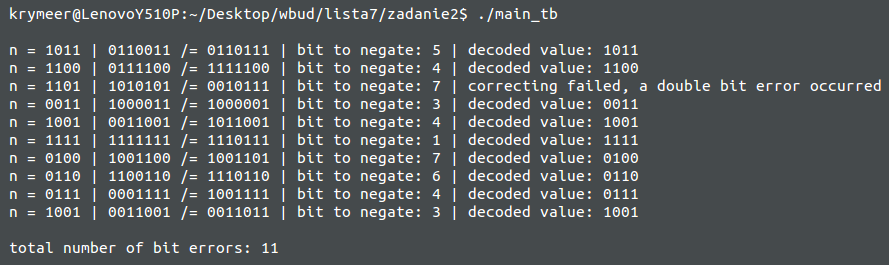
\includegraphics[width=1.2\textwidth,center]{output.png}
    \end{figure}

  Liczby z zakresu 0, 1... 15 zostały wysłane cztery razy, zatem kanał stratny przetransferował łącznie 64 ciągi czterobitowe. Dekoder kodu Hamminga wykrył 11 błędów, z czego 9 z nich udało się wyeliminować poprzez negację jednego z bitów (były to tzw. \textit{single bit errors}). Dla liczby $n=1101_2=13$ wystąpiły dwa przekłamania (kanał stratny zmienił bity 1. i 6.), w wyniku czego nie było możliwe naprawienie błędu -- koder Hamminga z 4 na 7 bitów potrafi wyeliminować i\,wykryć tylko jedno przekłamanie.

  \subsection{Przebiegi sygnałów}
  \begin{figure}[H]
    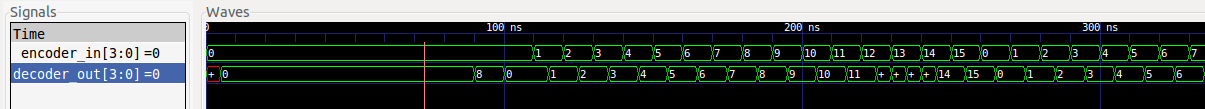
\includegraphics[width=1.2\textwidth,center]{gtk1.png}
    \caption{Liczby na wejściu i wyjściu kodera kodu Hamminga}
  \end{figure}
  W zapisie liczb 11, 12 i 13 w kodzie Hamminga zostały wykryte przekłamania, które dekoder próbował wyeliminować -- sygnał wyjściowy zmieniał się częściej niż zwykle. Dla 11 zmiana wartości nie była konieczna (zniekształcony bit był fragmentem kodu Hamminga).
  \begin{figure}[H]
    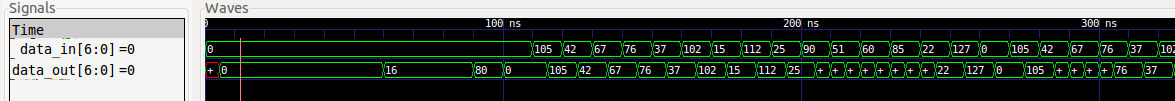
\includegraphics[width=1.2\textwidth,center]{gtk2.png}
    \caption{Liczby na wejściu i wyjściu kanału stratnego}
  \end{figure}
  Zakodowane postaci liczb 11, 12 i 13 uległy uszkodzeniu podczas transmisji za pośrednictwem kanału stratnego -- ich losowe bity zostały zamienione, co oczywiście skutkowało zmianą wartości na wyjściu.
  \begin{figure}[H]
    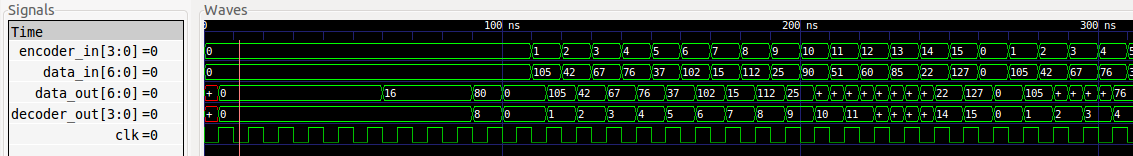
\includegraphics[width=1.2\textwidth,center]{gtk3.png}
    \caption{Zestawienie kodera i dekodera kodu Hamminga z kanałem stratnym}
  \end{figure}
  Pełny ,,cykl'': liczba na wejściu kodera kodu Hamminga $\rightarrow$ liczba na wejściu kanału stratnego $\rightarrow$ liczba na wyjściu kanału stratnego $\rightarrow$ liczba na wyjściu dekodera kodu Hamminga. Zmiany sygnałów wejściowych następują, gdy sygnał zegara zmienia się na \textit{'0'}, wyjściowych zaś -- kiedy wzrasta do \textit{'1'}.

\end{document}